\begin{frame}{Tiling}
    \begin{block}{Definition\hfill(\authcite{BeanPhd:phd})}
        A \emph{tiling} is a triple $\mathcal{T} = ((c,r), \mathcal{O}, \mathcal{R})$ where
        \begin{itemize}
            \item $(c,r) \in \Z^+ \times \Z^+$  is called \emph{dimension}
            \item $\mathcal{O} \subseteq \mathcal{G}^{(c,r)}$ is called \emph{obstructions}
            \item $\mathcal{R}=\set{\mathcal{R}_1,\mathcal{R}_2,\dotsc,\mathcal{R}_k} \subseteq \left(\mathcal{G}^{(c,r)}\right)^k$ is called \emph{requirements}
        \end{itemize}
    \end{block}
    \onslide<2->{The gridded permutations in $\textsf{Grid}(\mathcal{T})$ are those in $\mathcal{G}^{(c,r)}$ that 
    \begin{itemize}
        \item avoid $\mathcal{O}$
        \item contain $\mathcal{R}_1, \mathcal{R}_2, \dotsc, \mathcal{R}_k$
    \end{itemize}}
\end{frame}
\begin{frame}{Tiling - example}
    \begin{figure}
        \centering
        {
% rect
%\newcommand{\reqpnt}[3]{\fill[blue] (#1-#3,#2-#3) rectangle (#1+#3,#2+#3);}
% donut
%\newcommand{\reqpnt}[3]{\fill[blue] (#1,#2) circle (#3); \fill[white] (#1,#2) circle (#3 * 0.5);}
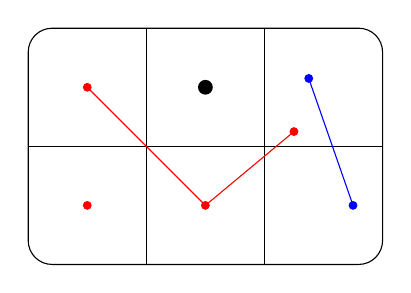
\begin{tikzpicture}[scale=0.75, every node/.style={scale=0.75}]
    \def\spnt{0.075} % Size of smaller points
    \def\lpnt{0.125} % Size of larger points
    \draw[rounded corners=2ex] (0,0) rectangle (6,4);
    \draw (2.0, 4) -- (2.0, 0);
    \draw (4.0, 4) -- (4.0, 0);
    \draw (0, 2) -- (6.0, 2);
    \fill[red] (1, 3) circle (\spnt);
    \fill[red] (1, 1) circle (\spnt);
    \fill[red] (3, 1) circle (\spnt);
    \fill[red] (4.5, 2.25) circle (\spnt);
    \draw[red] (1, 3) -- (3,1) -- (4.5,2.25);
    \fill (3,3) circle (\lpnt);
    \draw[blue] (4.75, 3.15) -- (5.5,1);
    \fill[blue] (4.75, 3.15) circle (\spnt);
    \fill[blue] (5.5, 1) circle (\spnt);
    %\reqpnt{4.75}{3.15}{\spnt*1.2}
    %\reqpnt{5.5}{1}{\spnt*1.2}
\end{tikzpicture}
}
        \caption{A tiling with $(c,r) = (3,2)$, $\mathcal{R} = \set{\set{1^{(1,1)}},\set{2^{(1,1)}1^{(2,0)}}}$ and $\mathcal{O} = \set{1^{(0,0)},12^{(1,1)},21^{(1,1)},3^{(0,1)}1^{(1,0)}2^{(2,1)}}$.}
    \end{figure}
\end{frame}